\documentclass[11pt,a4paper]{article}
\usepackage[margin=24mm]{geometry}\usepackage{fontspec,unicode-math,booktabs,graphicx,hyperref}
\setmainfont{STIXGeneral}\setmathfont{STIX Two Math}
\title{Gluing through a common point and along trees:\\complete manuscript costs}
\author{Human Compression project}\date{}
\begin{document}\maketitle
The original is Leemans--Mulpas, \emph{Two gluing methods for string C-group
representations of the symmetric groups}, arXiv:2504.17535v1, 24 April 2025
(register L010). All fifteen pages are counted, including references,
addresses and the identification banner. We compare them with both complete
common papers and the full application. The 23 source records describe one
original; the historical numerical sequence and unused preliminaries are
not claimed newly recovered.

\paragraph{The complete written comparison.}
For calibrated selected NFC characters without whitespace, the comparison is
\[
R_{\mathrm{written}}=\frac{27081}{12299+16117+11565}
=\frac{27081}{39981}=0.677347.
\]
The replacement written topic is longer in this coordinate. Both common
papers are charged once, with every proof, wrapper and reference passage.
The earlier Topic B umbrella is not used, and no overlap with another topic
is deducted.

\begin{center}\begin{tabular}{lrr}\toprule
Complete document&Pages&Characters\\\midrule
Original L010&15&27081\\
Common point paper $U_1$&5&12299\\
Synchronized tree paper $U_2$&6&16117\\
Application $A$&5&11565\\
Three diagnostic programs, printed&4&13371\\\bottomrule
\end{tabular}\end{center}

\paragraph{Programs and the conditional application.}
The full four-page program appendix gives the separate comparison
$R_{\mathrm{printed}}=27081/53352=0.507591$.
The three complete raw files cost 12768 characters and give
$R_{\mathrm{raw}}=27081/52749=0.513394$. These are alternative representations;
the printed and raw program costs are never added together. All three
programs validate examples and failed weakenings; none is a premise of the
uniform written theorems.

After acquiring \emph{both entire common papers and all three complete
declared programs}, the matched application comparison is
\[
r\mid(U_1,U_2,V)=\frac{27081}{11565}=2.341634.
\]
This is a conditional acquisition cost, not the whole-topic factor. The
three operational drivers cost 13578 characters separately; the two
Lean files cost 4214 and contain ten scoped declarations. They do not
formalize the complete source or its constructions.

\paragraph{What remains unpriced.}
Full costs of the retained endpoint sesquiextension theorem and classical
end-parabolic criterion are unknown. Historical software, complete formalization,
and the source diagrams' lines, incidence, colour and layout also remain
unknown, not zero. These figures measure available complete texts, not
minimum proof complexity or research effort. No new scientific credit is
assigned by this numerical packet.
\newpage
\begin{center}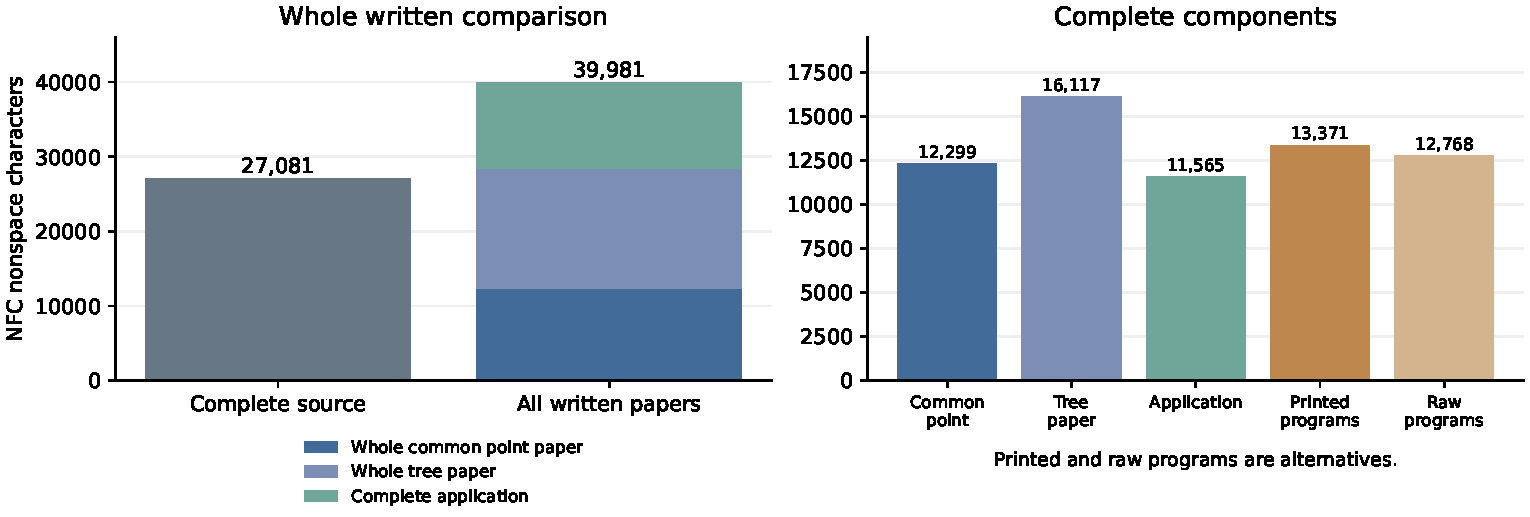
\includegraphics[width=\textwidth]{costs.pdf}\end{center}
\vspace{-3mm}
\begin{center}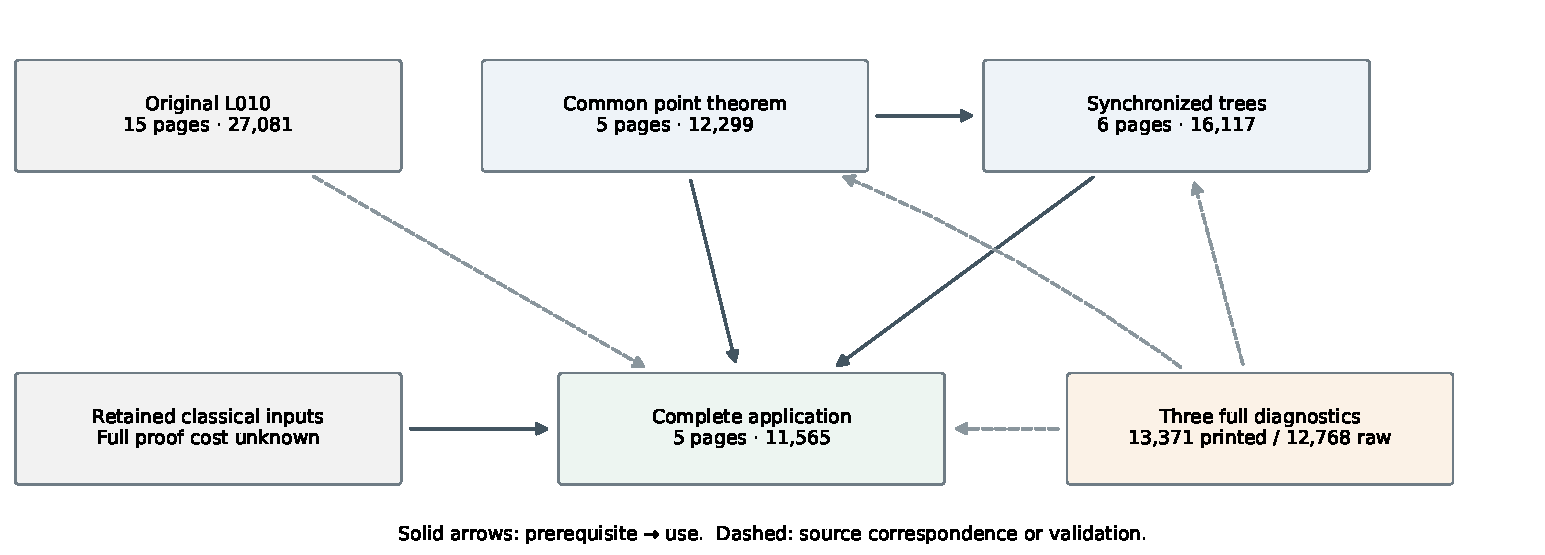
\includegraphics[width=\textwidth]{document_graph.pdf}\end{center}
\vspace{-4mm}
The graph shows complete-document dependencies. Each common paper is paid
once even when another paper uses it. Dashed validation and source links
are not proof prerequisites. Retained external proof costs stay unknown.
There is no node-count ratio or repeated-rise-and-fall claim.

\paragraph{Sensitivity to the unit of length.}
For calibrated selected NFC text, the whole written, program-inclusive
and conditional coordinates are:
\begin{center}\small\begin{tabular}{lrrrr}\toprule
Unit&Written&Printed&Raw&Conditional\\\midrule
Whitespace words & 0.803 & 0.713 & 0.721 & 2.734 \\
Alphanumeric units & 0.828 & 0.627 & 0.632 & 2.841 \\
Nonspace characters & 0.677 & 0.508 & 0.513 & 2.342 \\
Collapsed-space characters & 0.700 & 0.540 & 0.546 & 2.414 \\
Collapsed-space UTF-8 bytes & 0.673 & 0.531 & 0.537 & 2.326 \\
\bottomrule\end{tabular}\end{center}
All thirty coordinates are retained in JSON/CSV: five units under NFC and
NFKC, for complete raw extraction, furniture-only selection and calibrated
selection. Only isolated folios and exact running headers are removed in
selected text. Six observed glyph classes produce 175 substitutions; the
short stile is a separate encoded component. The curved code-wrap glyph
retains its literal comma. The unembedded banner is literal ASCII; unchanged
Type0 replacement text has no independent outline-equivalence claim.
Full graphical complexity remains outside these text coordinates.
\end{document}
